\section{Скользящее среднее и простая формула}
\textbf{Вопрос.} Садится ли среднее $\delta$ по оборотам на формулу $-\eta_1\delta_m^2/(2\eta_0)$ и на среднее нормальной формы?

Тот же запуск, $N=\vNlong$ оборотов. Формула берёт $\eta_0,\eta_1$ с магнитных элементов этого кольца и измеренную амплитуду $\delta_m$. Нормальная форма усредняет лабораторный $\delta$ по трём фазам того же произведения Ли и про имена $\eta,\xi$ не знает.

\begin{figure}[H]\centering
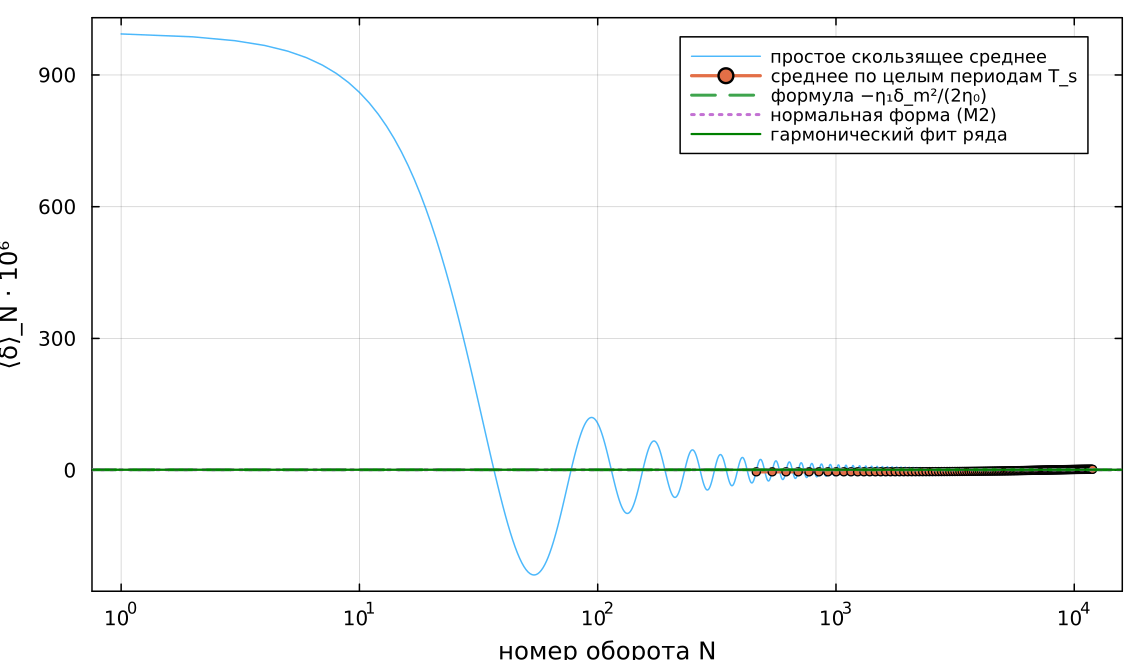
\includegraphics[width=0.92\textwidth]{figs/fig_02_runmean.png}
\caption{Простое среднее $\vMeanA$ и среднее по периодам $\vPmA$ ещё не сели. Гармонический фит $\vFitA$ (до формулы $\vDiffFitMone$). Формула $\vMoneA$, M2 $\vMtwoA$.}
\end{figure}

\textbf{Вывод.} Простое среднее за $\vNlong$ оборотов не село: сходится как $1/N$. Гармонический фит того же ряда садится на формулу и на M2. Между формулой и M2 разница $\vDiffAonetwo$.
